\section{Trace-Based Diagnostic Performance and Causal Inference Evolution (Scenario 4a and 4b)}
\label{sec:scenario4-results}

Scenario 4 evaluated the PANOPTES observability architecture coupled with a deterministic Trace-Based Root Cause Analysis (RCA) agent. The agent queried the Grafana Tempo REST API using TraceQL to isolate anomalous latency traces ($\ge 1500\,\text{ms}$) under the same $2000\,\text{ms}$ network degradation conditions applied in Scenario 3. To prevent state pollution and clock-drift artifacts, the agent utilized a Set-based state-tracking mechanism to strictly isolate novel faults from preexisting anomalous traces.

\subsection{Diagnostic Convergence and Accuracy}

Table~\ref{tab:s3_s4_comparison} contrasts the diagnostic outcomes between the Vanilla log-scraping baseline (Scenario 3) and the PANOPTES trace-driven agent (Scenario 4).

\begin{table}[htbp]
    \centering
    \caption{Comparative diagnostic outcomes: Vanilla (S3) versus PANOPTES (S4) over $N=30$ trials.}
    \label{tab:s3_s4_comparison}
    \begin{tabularx}{\textwidth}{l *{5}{>{\centering\arraybackslash}X}}
        \toprule
        \textbf{Scenario} & \textbf{Success ($Acc=1$)} & \textbf{Misattributed} & \textbf{Censored ($\ge 300\,\text{s}$)} & \textbf{Median $MTTDiag$} & \textbf{Mean $MTTDiag$} \\
        \midrule
        \textbf{S3: Vanilla}  & 5 ($16.67\%$) & 1 ($3.33\%$) & 24 ($80.00\%$) & $300.00\,\text{s}$ & $242.74 \pm 116.48\,\text{s}$ \\
        \textbf{S4: PANOPTES} & 7 ($23.33\%$) & 9 ($30.00\%$) & 14 ($46.67\%$) & $134.59\,\text{s}$ & $158.91 \pm 138.52\,\text{s}$ \\
        \bottomrule
    \end{tabularx}
\par\medskip\ABNTEXfontereduzida\selectfont\textbf{Source:} The author (2026) \par\medskip
\end{table}

A Fisher's Exact Test evaluating the diagnostic accuracy ($Acc$) between the two scenarios yielded $p = 0.748$, indicating no statistically significant improvement in the definitive root cause identification rate ($23.33\%$ versus $16.67\%$). The telemetry-rich PANOPTES architecture did not inherently resolve the accuracy deficit postulated in hypothesis $H_{1,2}$.

However, the structural nature of the diagnostic failures shifted dramatically. While the Vanilla scenario suffered from an $80.00\%$ right-censorship rate due to API polling exhaustion, the PANOPTES agent reduced censorship to $46.67\%$ but introduced a severe misattribution rate ($30.00\%$). Cross-tabulation of the empirical results reveals that the deterministic agent heavily misattributed faults to the \texttt{payment} microservice, regardless of whether the ground-truth fault was physically injected into \texttt{cart}, \texttt{shipping}, or \texttt{currency}.

This phenomenon highlights a fundamental boundary between data availability and causal inference. Because the Astronomy Shop checkout flow is highly coupled, a network delay in any downstream service inflates the end-to-end distributed trace duration. The naive deterministic agent checked for the mere presence of a service in the anomalous \texttt{serviceStats} array using a sequential loop over the candidate pool. Consequently, the first service evaluated (\texttt{payment}) was consistently flagged as the culprit if it participated in the degraded trace, bypassing the true root cause. 

\subsection{Diagnostic Latency and Telemetry Retrieval}

Despite the algorithmic misattributions, the PANOPTES architecture demonstrated a superior capability in accelerating telemetry retrieval. Figure~\ref{fig:scenarios_3_4_mttdiag} illustrates the comparative distribution of $MTTDiag$.

\begin{figure}[htbp]
    \centering
    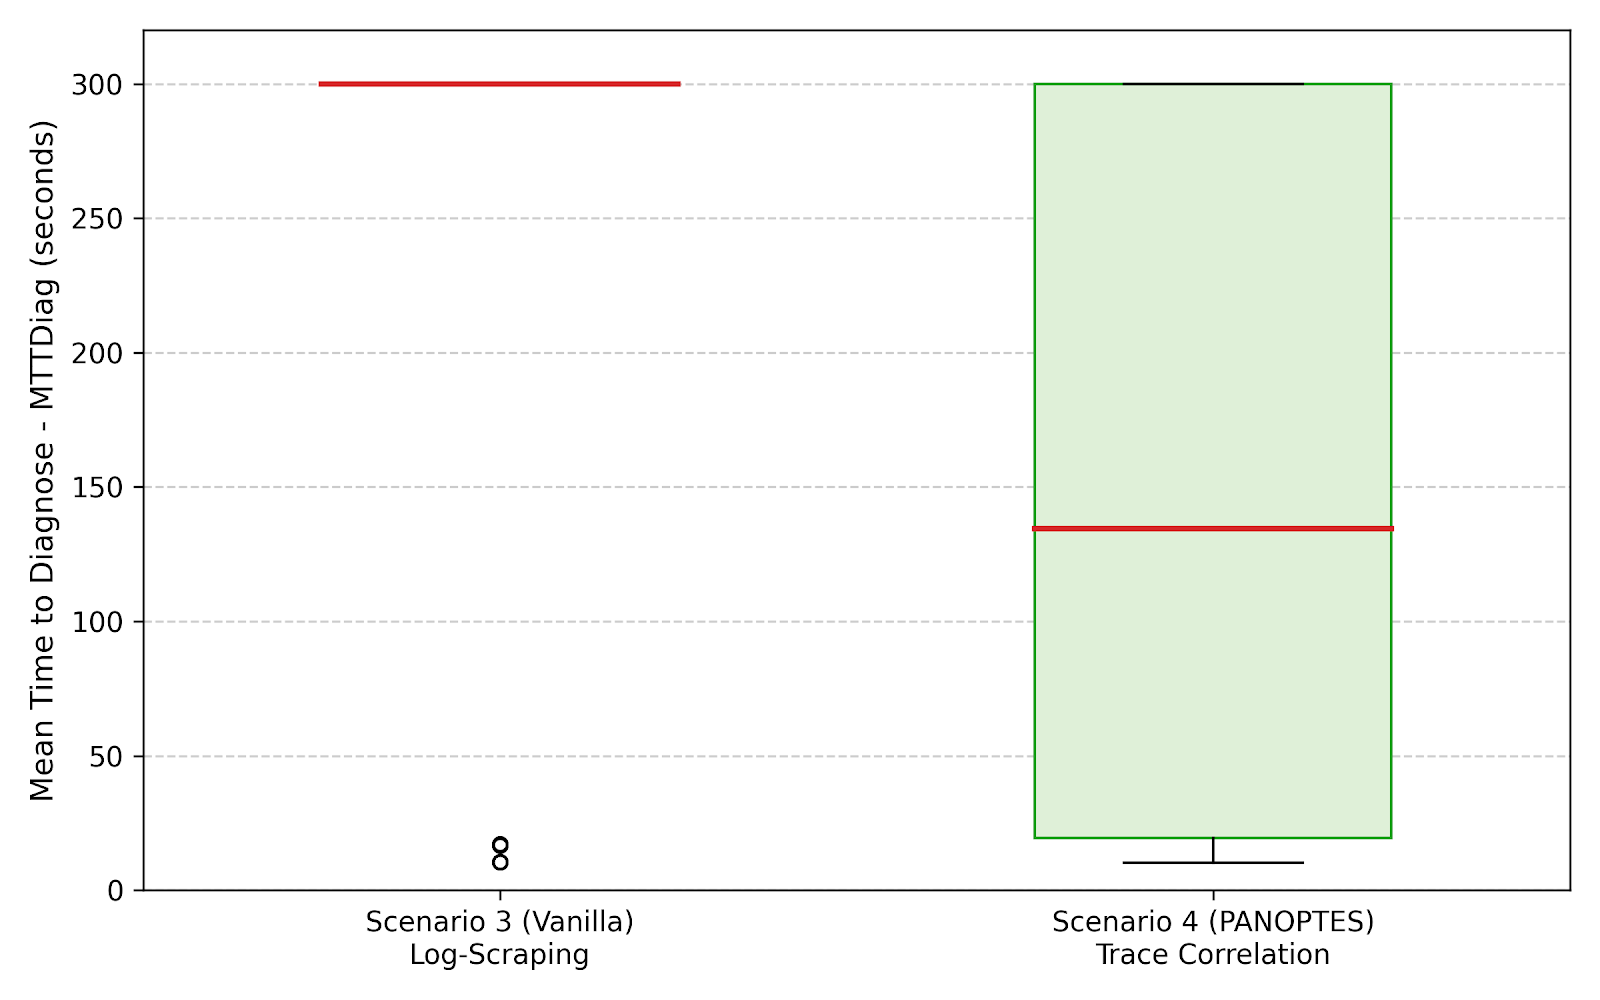
\includegraphics[width=0.85\textwidth]{images/results/scenarios_3_4_mttdiag_comparison.png}
    \caption{Distribution of $MTTDiag$ comparing Vanilla log-scraping versus PANOPTES trace correlation.}
    \label{fig:scenarios_3_4_mttdiag}
\end{figure}

A one-sided Mann-Whitney $U$ test confirmed that the PANOPTES agent converged significantly faster than the Vanilla baseline ($U = 309.0, \; p = 0.0081$). By replacing iterative local log scraping with indexed TraceQL queries, the median diagnostic latency dropped from $300.00\,\text{s}$ to $134.59\,\text{s}$, formally validating the hypothesis ($H_{1,1}$) that unified observability significantly reduces time-to-insight.

These results yield a critical conclusion for cloud-native reliability engineering: while unified observability pipelines (e.g., OpenTelemetry and Grafana Tempo) successfully eliminate the evidence retrieval bottleneck associated with distributed systems, they do not autonomously solve the causal attribution problem. To achieve high diagnostic accuracy, the RCA algorithm must move beyond binary trace-presence checks and evaluate the \textit{exclusive self-time} (critical path latency) of individual spans within the distributed trace graph.